\documentclass[a4paper, 12pt]{article}

\usepackage{amsfonts, amsmath, amssymb, amsthm}
\usepackage[english]{babel}
\usepackage[style=alphabetic]{biblatex}
\addbibresource{bibliography.bib}
\usepackage{csquotes}
\usepackage{enumitem}
\usepackage[a4paper,left=1.4cm,right=1.4cm,top=2cm,bottom=2cm]{geometry}
\usepackage[colorlinks=true, allcolors=blue]{hyperref}
\usepackage{mathtools}
\usepackage{nicematrix}
\usepackage{tikz}
\usetikzlibrary{shapes.multipart}
\usepackage[dvipsnames]{xcolor}

\setlength{\parindent}{0pt}
\newlength{\indentsize}
\setlength{\indentsize}{15pt}

\renewcommand{\thesubsubsection}{\alph{subsubsection})}

\newtheorem*{remark}{Remark}

% chktex-file 44

\title{\vspace{-0.6cm}Shortest Path Problem in Affine Subspaces}
\author{Charles Van Hees}
\date{\today}

\begin{document}
\maketitle

\vspace{-0.9cm}
\begin{abstract}
    In this short document, we describe the problem of finding the shortest path between a source $\mathbf{s}$ and a target $\mathbf{t}$, both in $\mathbb{R}^n$, while staying on affine subspaces $\{\mathbf{x} \in \mathbb{R}^n \vert A_i \mathbf{x} + b_i = 0\}, i = 1, \dots, m$. In the~\hyperref[sec:statement]{first section}, we introduce the problem and the notations used. Then, in section~\ref{sec:modelization}, we modelize it as a Shortest Path Problem (SPP) in a Graph of Convex Sets (GCS). We will explore two approaches for this. In the~\hyperref[sec:experiments]{last section}, we will discuss the pros and cons of both methods, based on experiments in Julia. It will be preceded by a theoretical discussion of the two models in section~\ref{sec:discussion}.
\end{abstract}

\section{Problem statement}\label{sec:statement}
\hspace{\indentsize} Let $\mathbf{s}, \mathbf{t} \in \mathbb{R}^n$ denote a source and a target respectively. Given a set of parameters \[{\left\{(A_i, b_i)\right\}}_{i=1}^{m} \subset \mathbb{R}^{d \times n} \times \mathbb{R}^d,\] we would like to find a path $q : [0,T] \mapsto \mathbb{R}^n$, with $q(0) = \mathbf{s}$ and $q(T) = \mathbf{t}$, such that, \[\forall \tau \in [0,T], \exists i \in \{1, \dots, m\} : A_i q(\tau) + b_i = 0.\] We will assume throughout this work that $\mathbf{s}$ and $\mathbf{t}$ belong to at least one of those affine subspaces. If it is not the case, trivially, such a path does not exist. The value of $T$ may be interpreted as the time at which we reach the target, or the length of the path between the source and the target.\\
In addition to this, we associate to each affine subspace a cost $\beta_i \in \mathbb{R}_{\geq 0}, i = 1, \dots, m$, representing the price to pay (per unity of measure) for staying on the corresponding affine subspace.

An example of such a problem in two dimensions is given in figure~\ref{fig:SPP-problem}.

\begin{figure}[!htb]
    \centering
    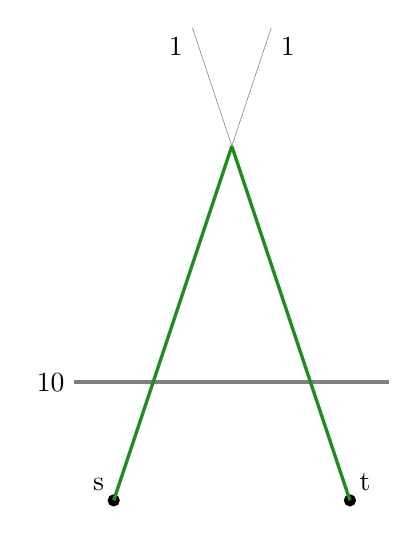
\begin{tikzpicture}
        \draw[gray, ultra thick] (-2,0) -- (2,0);
        \node[anchor=east] at (-2,0) {10};
        \draw[gray, very thin] (-0.5,4.5) -- (1.5,-1.5);
        \node[anchor=north east] at (-0.5,4.5) {1};
        \draw[gray, very thin] (-1.5,-1.5) -- (0.5,4.5);
        \node[anchor=north west] at (0.5,4.5) {1};

        \filldraw[black] (-1.5,-1.5) circle (2pt)
        node[anchor=south east] {s};
        \filldraw[black] (1.5,-1.5) circle (2pt)
        node[anchor=south west] {t};

        \draw[ForestGreen, very thick] (-1.5,-1.5) -- (0,3);
        \draw[ForestGreen, very thick] (0,3) -- (1.5,-1.5);
    \end{tikzpicture}
    \caption{Example of an SPP in which the path has to stay on given affine subspaces. We have three affine subspaces, of cost $10$, $1$ and $1$ respectively. The shortest path between the source $\mathbf{s}$ and the target $\mathbf{t}$ is represented in green. Notice the high cost of the horizontal line, preventing its utilization.}\label{fig:SPP-problem}
\end{figure}

\section{Modelization}\label{sec:modelization}
\hspace{\indentsize} In this section, we modelize mathematically the problem as a Shortest Path Problem (SPP) in a Graph of Convex Sets (GCS). GCS is a framework used to modelize graphs whose vertices are convex sets. It has been introduced in Tobia Marcucci's thesis~\cite{Tobia}, and may be used for several applications, like robot motion planning. The general model for SPP in GCS, with no cost on the vertices and nonnegative costs on the edges, is recalled in subsection~\ref{subsec:model}.\\
We see at least two ways to tackle this problem. The first one is by considering a graph whose vertices are given by the intersection of the affine subspaces, and the edges by the subspaces themselves. This first approach is expended in subsection~\ref{subsec:vertices}. An alternative, based on what is done in~\cite[Chapter~11]{Tobia} for motion planning, is to consider the subspaces as the vertices, binding two subspaces by an edge if they have an intersection. This is detailed in subsection~\ref{subsec:edges}.

\subsection{Model}\label{subsec:model}
\hspace{\indentsize} Let $\mathcal{G} = (\mathcal{V}, \mathcal{E})$ be a directed graph. To each vertex $v \in \mathcal{V}$, we associate a nonempty convex and compact set $\mathcal{X}_v \subset \mathbb{R}^p$. In the same way, to each edge $e = (v,w) \in \mathcal{E}$, we associate a nonempty convex and closed (not necessarily bounded) set $\mathcal{X}_e \subset \mathbb{R}^p \times \mathbb{R}^p$. In addition, a cost function $f_e : \mathbb{R}^p \times \mathbb{R}^p \mapsto \mathbb{R}$ is paired with each edge. We seek a path of minimal cost between a source $s \in \mathcal{V}$ and a target $t \in \mathcal{V}$. We assume here that there is no cost on the vertices and that the cost function $f_e$ is nonnegative. Thanks to these assumptions, the SPP on GCS can be modelized as\footnote{Details of how to obtain this model are available at~\cite[Chapters 5, 6 and 9]{Tobia}}~\cite[eq. 9.5]{Tobia}
\begin{subequations}\label{eq:vertices}
    \begin{align}
    \text{minimize}\quad   & \sum_{e = (v,w) \in \mathcal{E}} \tilde{f}_e (\mathbf{z}_v^e, \mathbf{z}_w^e, y_e)\label{eq:vertices-a}\\
    \text{subject to}\quad & y_e \in \{0, 1\} & \forall e \in \mathcal{E},\label{eq:vertices-b}\\
                           & \sum_{e \in \mathcal{I}_v^{in}} y_e + \delta_{sv} = \sum_{e \in \mathcal{I}_v^{out}} y_e + \delta_{tv} \leq 1 & \forall v \in \mathcal{V},\label{eq:vertices-c}\\
                           & \sum_{e \in \mathcal{I}_v^{in}} \mathbf{z}_v^e = \sum_{e \in \mathcal{I}_v^{out}} \mathbf{z}_v^e & \forall v \in \mathcal{V} \setminus \{s, t\},\label{eq:vertices-d}\\
                           & (\mathbf{z}_v^e, y_e) \in \tilde{\mathcal{X}}_v & \forall v \in \mathcal{V}, e \in \mathcal{I}_v,\label{eq:vertices-e}\\
                           & (\mathbf{z}_v^e, \mathbf{z}_w^e, y_e) \in \tilde{\mathcal{X}}_e & \forall e = (v,w) \in \mathcal{E}.\label{eq:vertices-f}
    \end{align}
\end{subequations}
where $\tilde{f}_e$, $\tilde{\mathcal{X}}_v$ and $\tilde{\mathcal{X}}_e$ are the closures of the homogenizations\footnote{In what follows, the term \textit{closure} will often be omitted, even if it will implicitly be considered as such.} of $f_e$, $\mathcal{X}_v$ and $\mathcal{X}_e$ respectively, and \[\delta_{vw} = \begin{cases} 1 & \text{ if } v = w\\ 0 & \text{ otherwise}\end{cases} \qquad \forall v,w \in \mathcal{V}.\]

For all $v \in \mathcal{V}$, the sets $\mathcal{I}_v^{in}$, $\mathcal{I}_v^{out}$ and $\mathcal{I}_v$ denote the sets of incoming edges to $v$, outgoing edges, and the union of incoming and outgoing edges respectively.

\hspace{\indentsize} We distinguish three different kind of variables:
\begin{itemize}
    \item $\mathbf{x}_v \in \mathbb{R}^p$ for all $v \in \mathcal{V}$, which are continuous variables corresponding to the position of a point in the convex set of node $v$. These variables are constrained in the sets $\mathcal{X}_v$ if the shortest path goes through node $v$, which is hidden in the constraint~(\ref{eq:vertices-e});
    \item $y_e \in \{0,1\}$ for all $e \in \mathcal{E}$, which are binary variables, corresponding to the choice of taking the edge $e$ or not in the path;
    \item $\mathbf{z}_v^e \in \mathbb{R}^p$ for all $e \in \mathcal{I}_v$, for all $v \in \mathcal{V}$, which are auxiliary variables corresponding to the product of the two previous variables.
\end{itemize}
Notice that the variables $\mathbf{x}_v$ do not appear in model~(\ref{eq:vertices}), and the only decision variables that need to be given to the solver are $y_e$ and $\mathbf{z}_v^e$. We may then recover the values of the variables $\mathbf{x}_v$ at the vertices of the path as the value of $\mathbf{z}_v^e$ for an incident edge in the path (i.e., for which $y_e = 1$).

\hspace{\indentsize} Constraints~\ref{eq:vertices-c} and~\ref{eq:vertices-d} can be seen as flow conservation equations, i.e., if a vertex is entered, then the path has to exit it. The $\delta_{ij}$ function defined above allows to have a virtual unit entering the source $s$ and exiting the target $t$. The upper bound of $1$ in~\ref{eq:vertices-c} is to ensure that a vertex is not entered twice, and is called the degree constraint. Finally, the constraint~\ref{eq:vertices-f} ensures that the edges belong to $\mathcal{X}_e$.

\begin{remark} The dimension $p$ used here above to define the set $\mathcal{X}_v$ may be equal to the dimension $n$ of the problem defined in section~\ref{sec:statement} (like in subsection~\ref{subsec:vertices}), but has not to be equal (like in~\ref{subsec:edges}).\end{remark}

\subsection{Intersections as vertices}\label{subsec:vertices}
\hspace{\indentsize} The first possibility is to construct a graph whose vertices are the intersections between affine subspaces, and whose edges are the affine subspaces, i.e., there is an edge between two vertices if they belong to a same affine subspace. In addition, we put a weight on each edge, corresponding to the cost of the affine subspace binding the two intersections. Furthermore, all the edges are duplicated, in order to have a directed graph (the undirected edge between vertices $v$ and $w$ is transformed into one edge from $v$ to $w$ and one edge from $w$ to $v$).\\
We add to this graph two vertices, one for the source $s$ and one for the target $t$, associated with the singleton corresponding to there coordinates. Those are binded to the vertices corresponding to subspaces of the affine subspaces to which they belong, with a simple directed edge (no need to come back to the source or to go out of the target). Again, a weight is put on these edges, being the cost of the corresponding affine subspace.\\
For example, the GCS corresponding to the problem of figure~\ref{fig:SPP-problem} is drawn in figure~\ref{fig:vertices}. There are five vertices, corresponding to the three intersections, the source and the target.

\begin{figure}[!htb]
    \centering
    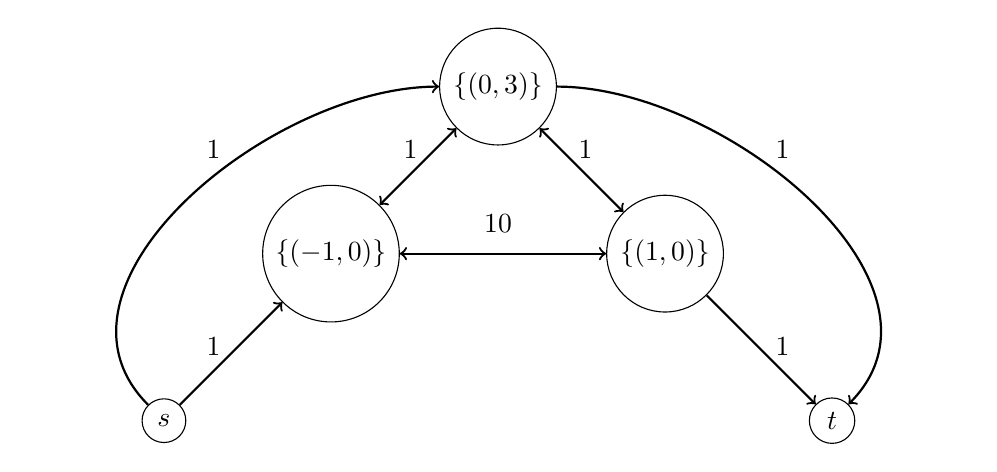
\begin{tikzpicture}[node distance={3cm}]
        \node[draw, circle] (1) {$\{(0,3)\}$};
        \node[draw, circle] (2) [below left of=1] {$\{(-1,0)\}$};
        \node[draw, circle] (3) [below right of=1] {$\{(1,0)\}$};
        \node[draw, circle] (4) [below left of=2] {$s$};
        \node[draw, circle] (5) [below right of=3] {$t$};

        \draw[thick, <->] (1) to (2); \node[anchor=east] at (-0.9,-0.8) {1};
        \draw[thick, <->] (1) to (3); \node[anchor=west] at (0.9,-0.8) {1};
        \draw[thick, <- ] (1) to [out=180, in=135, looseness=1] (4); \node[anchor=east] at (-3.4,-0.8) {1};
        \draw[thick,  ->] (1) to [out=0, in=45, looseness=1] (5); \node[anchor=west] at (3.4,-0.8) {1};
        \draw[thick, <->] (2) to (3); \node[anchor=north] at (0,-1.5) {10};
        \draw[thick, <- ] (2) to (4); \node[anchor=east] at (-3.4,-3.3) {1};
        \draw[thick,  ->] (3) to (5); \node[anchor=west] at (3.4,-3.3) {1};
    \end{tikzpicture}
    \caption{GCS corresponding to the problem presented in figure~\ref{fig:SPP-problem}, with the intersections as vertices. The coordinates of the intersection points are there only for an illustration purpose.}\label{fig:vertices}
\end{figure}

\hspace{\indentsize} Let us now describe mathematically all the components of this problem. To each vertex $v \in \mathcal{V}\setminus\{s,t\}$, we associate the convex region corresponding to the intersection of the two corresponding subspaces (let us say $i$ and $j$). This set is nonempty, closed, but not bounded. Therefore, we add an $L_{\infty}$-ball of radius $R$ large enough. The set $\mathcal{X}_v$ can subsequently be described by \[\mathcal{X}_v \coloneq \left\{\mathbf{x} \in \mathbb{R}^n \left\lvert \begin{bmatrix} A_i \\ A_j \end{bmatrix} \mathbf{x} + \begin{bmatrix} b_i \\ b_j \end{bmatrix} = 0, {\lVert \mathbf{x} \rVert}_\infty \leq R \right.\right\}.\]

The homogenization of this set is~\cite[eq. 2.5]{Tobia} \[\tilde{\mathcal{X}}_v \coloneq \left\{(\mathbf{x},y) \in \mathbb{R}^n \times \mathbb{R}_{\geq 0} \left\lvert \begin{bmatrix} A_i \\ A_j \end{bmatrix} \mathbf{x} + y \begin{bmatrix} b_i \\ b_j \end{bmatrix} = 0, {\lVert \mathbf{x} \rVert}_\infty \leq Ry \right.\right\}.\]

For the source and the target, the sets $\mathcal{X}_s$ and $\mathcal{X}_t$ are easily described by their respective coordinates: \[\mathcal{X}_s \coloneq \{\mathbf{x} \in \mathbb{R}^n \left\lvert \mathbf{x} = \mathbf{s}\right.\} \qquad \mathcal{X}_t \coloneq \{\mathbf{x} \in \mathbb{R}^n \left\lvert \mathbf{x} = \mathbf{t}\right.\}.\]

Their homogenizations are given by
\begin{equation}\label{eq:homogenizationSourceTarget}
    \tilde{\mathcal{X}}_s \coloneq \{(\mathbf{x},y) \in \mathbb{R}^n \times \mathbb{R}_{\geq 0} \left\lvert \mathbf{x} = \mathbf{s} y \right.\} \qquad \tilde{\mathcal{X}}_t \coloneq \{(\mathbf{x},y) \in \mathbb{R}^n \times \mathbb{R}_{\geq 0} \left\lvert \mathbf{x} = \mathbf{t} y \right.\}.
\end{equation}

\hspace{\indentsize} Let $v$ and $w$ be two nodes of the graph, associated with the convex regions $\mathcal{X}_v$ and $\mathcal{X}_w$ respectively, and linked by an edge $e$ of weight $\beta$. The convex cost function on the edges is defined as
\begin{equation*}\label{eq:f_e}
    f_e(\mathbf{x}_v, \mathbf{x}_w) = \beta {\lVert \mathbf{x}_v - \mathbf{x}_w \rVert}_2.
\end{equation*}
Its homogenization is given by
\begin{equation*}
    \tilde{f}_e(\mathbf{x}_v, \mathbf{x}_w, y) \quad = \quad \begin{cases} \beta {\lVert \mathbf{x}_v - \mathbf{x}_w \rVert}_2 & \quad \text{if $y > 0$} \\ \infty & \quad \text{if $y = 0$}\end{cases},
\end{equation*}
with $\tilde{f}_e(\mathbf{0}, \mathbf{0}, 0) = 0$.\\
Notice that, with this modelization, there is no constraint on the edges. Hence, $\mathcal{X}_e \coloneq \mathbb{R}^n \times \mathbb{R}^n$, and constraint~\ref{eq:vertices-f} is useless.

\subsection{Intersections as edges\protect\footnote{Largely inspired from~\cite[Chapter 11.2]{Tobia}}}\label{subsec:edges}
\hspace{\indentsize} The second option is to consider the intersections of affine subspaces as the edges, and taking for vertices the affine subspaces themselves, plus the source and the target. The source and target are linked by an edge to the subspace (potentially several) they are contained in. Again, we consider a directed graph by duplicating all the edges between two vertices different from the source and the target. Finally, we associate to each vertex different from the source and the target the cost associated with the affine subspace. The corresponding GCS of the problem of figure~\ref{fig:SPP-problem} is drawn in figure~\ref{fig:edges}.

\begin{figure}[!htb]
    \centering
    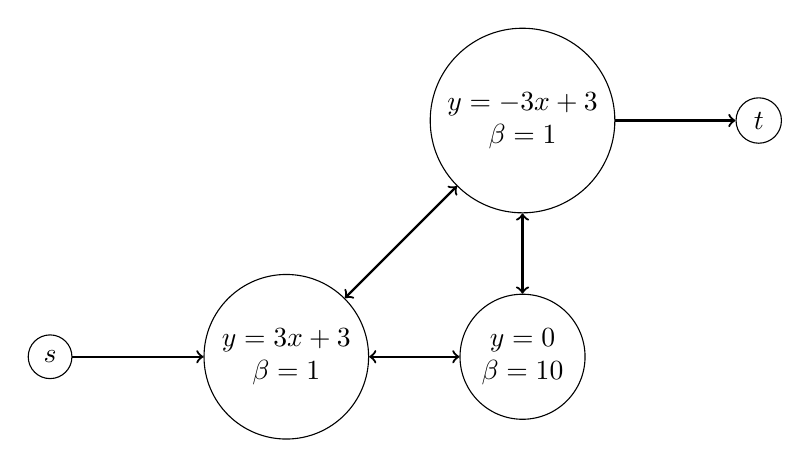
\begin{tikzpicture}[node distance={3cm}, every text node part/.style={align=center}]
        \node[draw, circle] (1) {$s$};
        \node[draw, circle] (2) [right of=1] {$y = 3x + 3$ \\ $\beta = 1$};
        \node[draw, circle] (3) [right of=2] {$y = 0$ \\ $\beta = 10$};
        \node[draw, circle] (4) [above of=3] {$y = -3x + 3$ \\ $\beta = 1$};
        \node[draw, circle] (5) [right of=4] {$t$};

        \draw[thick,  ->] (1) to (2);
        \draw[thick, <->] (2) to (3);
        \draw[thick, <->] (2) to (4);
        \draw[thick, <->] (3) to (4);
        \draw[thick,  ->] (4) to (5);
    \end{tikzpicture}
    \caption{GCS corresponding to the problem presented in figure~\ref{fig:SPP-problem}, with the intersections of subspaces as edges.}\label{fig:edges}
\end{figure}

\hspace{\indentsize} For each affine subspace $i = 1, \dots, m$, we define the convex region \[\mathcal{C}_i \coloneq \{\mathbf{x} \in \mathbb{R}^n \mid A_i \mathbf{x} + b_i = 0, {\lVert \mathbf{x} \rVert}_\infty \leq R\}.\]
Again, $R$ is chosen big enough, and the $L_\infty$-ball is there to bound the set. Then, we associate to each vertex $v \in \mathcal{V}\setminus\{s, t\}$ the convex constraint set $\mathcal{X}_v \coloneq \mathcal{C}_i \times \mathcal{C}_i$, where $i$ corresponds to the index of the affine subspace associated to node $v$. The points inside those sets can be seen as pairs of two points in the affine subspace: the starting point and the ending point. Mathematically, $\mathbf{x}_v \coloneq (\mathbf{q}_{v,0}, \mathbf{q}_{v,1})$, with $\mathbf{q}_{v,0}, \mathbf{q}_{v,1} \in \mathbb{R}^n$. The homogenization of the set $\mathcal{X}_v$ is given by \[\tilde{\mathcal{X}}_v \coloneq \{(\mathbf{q}_{v,0}, \mathbf{q}_{v,1}, y) \in \mathbb{R}^n \times \mathbb{R}^n \times \mathbb{R}_{\geq 0} \left\lvert A_i \mathbf{q}_{v,0} + b_i y = A_i \mathbf{q}_{v,1} + b_i y = 0, {\lVert \mathbf{q}_{v,0} \rVert}_\infty \leq Ry, {\lVert \mathbf{q}_{v,1} \rVert}_\infty \leq Ry \right.\}\]
We associate a cost function on those vertices, being the euclidean distance between the two points, multiplied by the cost of the affine subspace: \[f_v(\mathbf{x}_v) = \beta_v {\lVert \mathbf{q}_{v,0} - \mathbf{q}_{v,1} \rVert}_2, \qquad \forall v \in \mathcal{V}.\]
For the source $s$ and the target $t$, we define $\mathcal{X}_s$ and $\mathcal{X}_t$ in the same way as in subsection~\ref{subsec:vertices}, and their homogenization are given by~\ref{eq:homogenizationSourceTarget}. No cost is associated to those vertices.

\hspace{\indentsize} Having a cost on the vertices is problematic, as the model~\ref{eq:vertices} is defined for a graph with no cost on the vertices, and nonnegative costs on the edges. To solve this problem, we are going to transfer the cost from the vertices to the edges outgoing the vertices. I.e., for each edge $e = (v,w) \in \mathcal{E}$, we associate the cost function\footnote{To be fully rigorous, we should not take the edges outgoing the source.} \[f_e(\mathbf{q}_{v,0}, \mathbf{q}_{v,1}, \mathbf{q}_{w,0}, \mathbf{q}_{w,1}) = \beta_v {\lVert \mathbf{q}_{v,0} - \mathbf{q}_{v,1} \rVert}_2.\]

Finally, to ensure the continuity of the path, we impose a constraint on the edges by associating them to the convex set\footnote{Again, for rigor, when $v = s$, we may replace $\mathbf{q}_{v,0}$ and $\mathbf{q}_{v,1}$ by $\mathbf{q}_s$. Similarly, when $w = t$, we may replace $\mathbf{q}_{w,0}$ and $\mathbf{q}_{w,1}$ by $\mathbf{q}_t$.} \[\mathcal{X}_e \coloneq \{(\mathbf{q}_{v,0}, \mathbf{q}_{v,1}, \mathbf{q}_{w,0}, \mathbf{q}_{w,1}) \in \mathbb{R}^{4n} \mid \mathbf{q}_{v,1} = \mathbf{q}_{w,0}\} \qquad \forall e = (v,w) \in \mathcal{E}.\]
The homogenization of this set is given by \[\tilde{\mathcal{X}}_e \coloneq \{(\mathbf{q}_{v,0}, \mathbf{q}_{v,1}, \mathbf{q}_{w,0}, \mathbf{q}_{w,1}, y) \in \mathbb{R}^{4n} \times \mathbb{R}_{\geq 0} \mid \mathbf{q}_{v,1} = \mathbf{q}_{w,0}\} \qquad \forall e = (v,w) \in \mathcal{E}.\]

\begin{remark} This modelization has a major drawback: it does not allow the path to take two times the same affine subspace. We could duplicate the affine subspaces to deal with that problem, at the cost of increasing the size of the graph. If an affine subspace intersects $\delta$ other subspaces, we should have $\lceil \delta/2 \rceil$ copies of the affine subspace.\end{remark}

\section{Discussion}\label{sec:discussion}
\subsection{$L_\infty$-ball}
The choice of the center and of the radius of the ball is crucial: how to be sure it is large enough to capture the optimal solution, while staying small enough to avoid numerical issues?~\cite{Radius}

First, we should check the feasibility of the problem. For this, we have two options. The first one is to discard the ball constraint. The solver will find a solution if and only if there is a path between the source and the target staying on the given affine subspaces. This is ensured by the construction of the graph and by the constraint~\ref{eq:vertices-c}. In fact, a much easier way is to consider the standard graph $\mathcal{G} = (\mathcal{V}, \mathcal{E})$ given by the same nodes and edges as our GCS, and to verify the existence of a path between the source and the target, using an algorithm like Depth-First Search of Breadth-First Search.

Once we are sure of the existence of a path between the source and the target, we can try to minimize the cost along this path, using one of the two models defined previously. First, we can put the center of the ball at the middle point between the source and the target, and set $R$ to some arbitrary small value (e.g. $1$). As long as the solver does not find a solution, we can multiply $R$ by a factor $\alpha$ (possibly non constant). Once a solution is found, its value $U$ is an upper bound on the optimal value. Using this upper bound, we can find the optimal center and radius of the ball, i.e., the ones minimizing the radius and for which we are sure to find the optimal solution. Those values can be obtained by solving the following minimax\footnote{Intuitively, we would like to find the center of the ball that will minimize the worst case, 
It is a maximization problem as we would like to find the worst case. Using the optimal $R^*$ of this maximization problem will ensure that the optimal solution is in the ball of radius $R^*$.} problem:
\begin{subequations}\label{eq:ball}
    \begin{align}
        \min_{\mathbf{x} \in \mathbb{R}^n} \max_{\substack{R \in \mathbb{R}_{\geq 0} \\ \alpha, \beta \in \mathbb{R}_{\geq 0}}} &&& R\label{eq:ball-a}\\
        s.t. &&& \alpha = \min_{i=1, \dots, m} \left\{\sqrt{{(x_i + R - s_i)}^2 + \sum_{\substack{j = 1 \\ j \neq i}}^{d}{\left(\frac{t_j - s_j}{2}\right)}^2} + \sqrt{{(x_i + R - t_i)}^2 + \sum_{\substack{j = 1 \\ j \neq i}}{\left(\frac{t_j - s_j}{2}\right)}^2}\right\}\label{eq:ball-b}\\
             &&& \beta = \min_{i=1, \dots, m} \left\{\sqrt{{(x_i - R - s_i)}^2 + \sum_{\substack{j = 1 \\ j \neq i}}^{d}{\left(\frac{t_j - s_j}{2}\right)}^2} + \sqrt{{(x_i - R - t_i)}^2 + \sum_{\substack{j = 1 \\ j \neq i}}{\left(\frac{t_j - s_j}{2}\right)}^2}\right\}\label{eq:ball-c}\\
             &&& \min \{\alpha, \beta\} \leq U\label{eq:ball-d}
    \end{align}
\end{subequations}

By symmetry, the center $\mathbf{x}$ of the ball should be the mean of the source and target coordinates. Setting $\mathbf{x} = \frac{\mathbf{s} + \mathbf{t}}{2}$ in~\ref{eq:ball-b} and~\ref{eq:ball-c}, we get $\alpha = \beta$. Furthermore, constraint~\ref{eq:ball-d} will be tight at the optimal point. Hence, we are looking to a nonnegative value of $R$ such that \[U = \min_{i=1, \dots,  m} \left\{ \sqrt{{\left(R + \frac{t_i - s_i}{2}\right)}^2 + \sum_{\substack{j=1 \\ j \neq i}}^{d} {\left(\frac{t_j - s_j}{2}\right)}^2} + \sqrt{{\left(R + \frac{s_i - t_i}{2}\right)}^2 + \sum_{\substack{j=1 \\ j \neq i}}^{d} {\left(\frac{t_j - s_j}{2}\right)}^2}\right\}.\]

\subsection{Structure of the graphs}
We define by $p$ the number of intersections of affine subspace in the problem. Recall that $m$ is the number of affine subspaces, and $n$ is the dimension of the space. Furthermore, for each affine subspace $i = 1, \dots, m$, we let $\delta_i$ be the number of affine subspaces it intersects. Notice that $2p = \sum_{i=1}^m \delta_i$.\\
We will analyse the number of vertices and edges of the graphs of both modelization. Based on this, we will be able to find the number of binary and continuous variables, and of constraints, in the optimization problem. In what follows, we neglect the vertices and edges associated to the source and target, as those are generally marginal with respect to the rest.

\subsubsection{Intersections as vertices}
When we take the intersections of affine subspaces as the vertices of the graph, we have $|\mathcal{V}| = p$ vertices. The number of edges is \[|\mathcal{E}| = \sum_{i=1}^m \delta_i (\delta_i - 1) = \left(\sum_{i=1}^m {\delta_i}^2 - \sum_{i=1}^m \delta_i\right).\] To see this, consider the intersection between affine subspaces $i$ and $j$. The number of edges incident to the corresponding node is equal to $(\delta_i - 1) + (\delta_j - 1)$. Therefore, we can consider the increments of the two affine subspaces separately. Since affine subspace $i$ has $\delta_i$ intersections, its total contribution is $\delta_i (\delta_i - 1)$. And this is valid for all $i \in \{1, \dots, m\}$. With this, all the edges are counted two times, as desired for the directed graph.

From this, we can infer that there are $|\mathcal{E}|$ binary variables, and $2n|\mathcal{E}|$ continuous variables. The constraints are as follow:
\begin{itemize}[label={}, leftmargin=0.5cm]
    \item~\ref{eq:vertices-c} implies $|\mathcal{V}|$        constraints;
    \item~\ref{eq:vertices-d} implies $n|\mathcal{V}|$       constraints;
    \item~\ref{eq:vertices-e} implies $2|\mathcal{E}|$ times $(2d+n)$ constraints.
\end{itemize}
Hence, the total number of constraints is \[(1+n)p + 2(2d+n) \left(\sum_{i=1}^m {\delta_i}^2 - \sum_{i=1}^m \delta_i\right).\]

\subsubsection{Intersections as edges}
When the affine subspaces are chosen to be the vertices of the graph, we have $|\mathcal{V}| = m$ vertices and \[|\mathcal{E}| = 2p = \sum_{i=1}^{m} \delta_i\] edges (as all the edges are duplicated to create a directed graph). This implies $|\mathcal{E}|$ binary variables, for $4n|\mathcal{E}|$ continuous variables. Let us now count the number of constraints:
\begin{itemize}[label={}, leftmargin=0.5cm]
    \item~\ref{eq:vertices-c} corresponds to $|\mathcal{V}|$   constraints;
    \item~\ref{eq:vertices-d} corresponds to $2n|\mathcal{V}|$ constraints;
    \item~\ref{eq:vertices-e} corresponds to $2|\mathcal{E}|$ times $2(d+n)$ constraints;
    \item~\ref{eq:vertices-f} corresponds to $n|\mathcal{E}|$  constraints.
\end{itemize}
The total number of constraints is therefore \[(1+2n)m + 2(4d+5n)p.\]

\subsection{Comments}
Based on this complexity analysis, the modelization to use seems to be problem-dependent.

\section{Numerical experiments}\label{sec:experiments}
The implementation of these two models is available at \url{https://github.com/CharlesVanHees/SPPAffineSubspaces}.

\printbibliography{}
\end{document}